\documentclass[border=0.1cm]{standalone}
\usepackage{tikz}
\usetikzlibrary{arrows, arrows.meta}

\tikzset{
    node1/.style={
        above right
    }
}
\begin{document}
    \begin{tikzpicture}
        \node[node1,label={\LARGE $A \cup B$}] at (0,0)
        {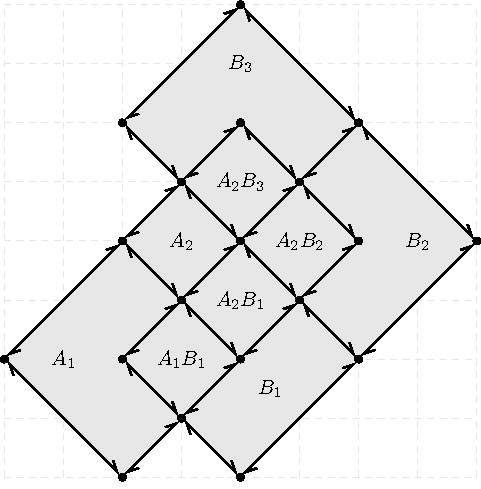
\includegraphics[scale=0.75]{DCELUnion}};
        \node[node1,label={\LARGE $A \cap B$}]           at (7,0)  {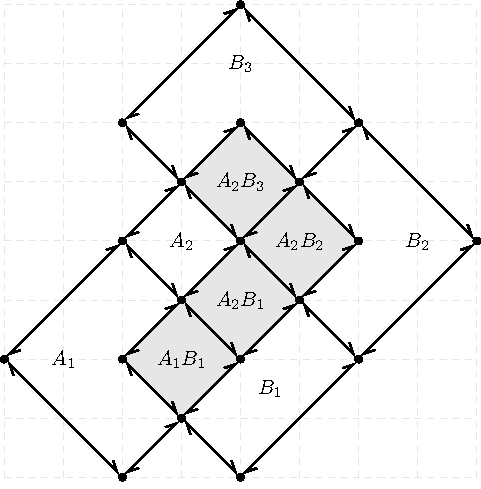
\includegraphics[scale=0.75]{DCELIntersection}};
        \node[node1,label={\LARGE $A \setminus B$}]      at (14,0) {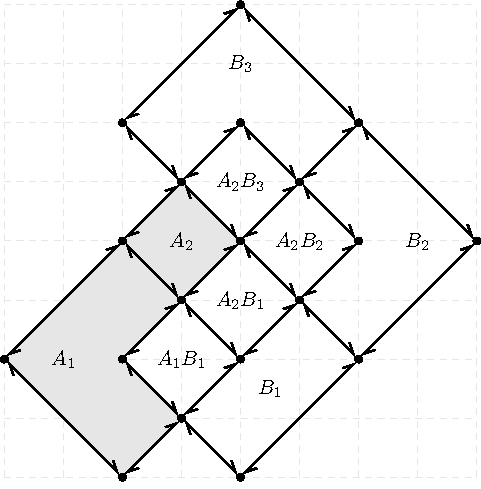
\includegraphics[scale=0.75]{DCELDiffA}};
        \node[node1,label={\LARGE $B \setminus A$}]      at (21,0) {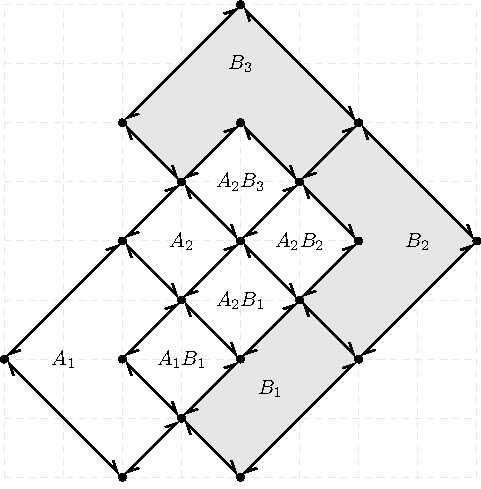
\includegraphics[scale=0.75]{DCELDiffB}};
        \node[node1,label={\LARGE $A \bigtriangleup B$}] at (28,0) {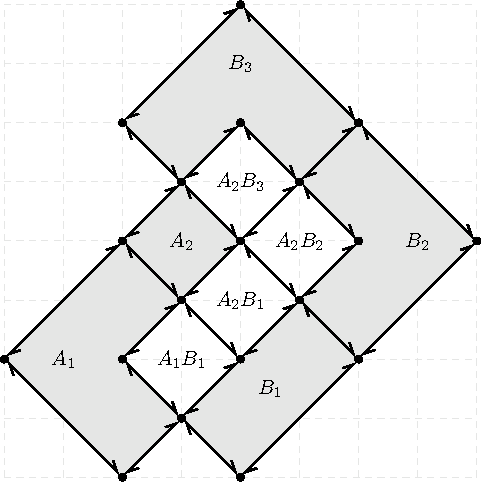
\includegraphics[scale=0.75]{DCELDiff}};
    \end{tikzpicture}
\end{document}
